% Research proposal: mechanism of cross-modal leakage after unimodal unlearning in VLMs.
% Figure: figures/lens_step75.pdf (scripts/plot_umu_lens.py on results/llava/mech_umu/umu_npo_txt_lr5e-05_s0/step75/lens.json).
% Numbers come from the repo's runs (DEVIATIONS.md DEV-011, DEV-012; Drive runs/llava/umu_unlearn/,
% results/llava/mech_umu/). Citations marked % VERIFY are taken from research.md and must be checked against
% the papers before submission.
\documentclass[11pt]{article}
\usepackage[margin=1in]{geometry}
\usepackage[T1]{fontenc}
\usepackage{lmodern}
\usepackage{microtype}
\usepackage{amsmath,amssymb}
\usepackage{booktabs}
\usepackage{tabularx}
\usepackage{enumitem}
\usepackage{xcolor}
\usepackage{graphicx}
\usepackage[colorlinks=true,linkcolor=black,citecolor=black,urlcolor=blue!50!black]{hyperref}

\newcommand{\Hone}{\textbf{H1}}
\newcommand{\Honep}{\textbf{H1$'$}}
\newcommand{\Htwo}{\textbf{H2}}
\newcommand{\thu}{\theta_u}
\newcommand{\tho}{\theta_0}
\setlist{itemsep=2pt,topsep=4pt}

\title{Why Unlearned Knowledge Leaks Across Modalities:\\
A Causal, Layer-wise Analysis of Text-only Unlearning in Vision--Language Models}
\author{Xuzhong Wang}
\date{Research proposal and progress report --- 5 November 2026}

\begin{document}
\maketitle

\begin{abstract}
When a vision--language model (VLM) is made to forget a fact through text-only questions, the fact often
remains answerable when the same entity is shown as an image. This leakage, and its asymmetry
(text$\to$image leaks more than image$\to$text), has been reported behaviourally, but no work has intervened
causally inside the \emph{unlearned} model to explain it. We propose to discriminate three pre-registered
mechanisms --- late-layer input-form gating (\Hone), early-layer route separation (\Honep), and
suppression followed by compensation (\Htwo) --- with the logit lens, layer-wise LoRA masking, a
decomposition of the LoRA update $\lVert\Delta W x\rVert$ by token group, and cross-route activation
patching. On UMU-Bench with LLaVA-1.5-7B we have (i)~reproduced the benchmark's vanilla model exactly,
(ii)~found that the standard letter-logit multiple-choice readout badly underestimates what that model knows,
(iii)~produced a strong text$\to$image leak with text-only NPO ($G = 0.385$ after one epoch), and (iv)~a first
logit-lens result: the text route is suppressed in the layers where the answer emerges (L20--24), the image
route is almost untouched there, and adding the portrait to a name-based question removes the suppression.
The last finding argues against strong compensation (\Htwo) and suggests that, in this model, the gate is
the \emph{absence of an image} rather than the name. We describe the experiments that will test this.
\end{abstract}

%===========================================================================================================
\section{Problem and research question}

Machine unlearning for multimodal models is usually evaluated in the modality it was applied in. Recent
benchmarks show that this is not enough: after text-only unlearning, the same knowledge can still be
retrieved from an image of the entity, and the transfer is asymmetric. UNLINK-VL reports, on real
(pre-trained) entities with strictly paired questions, that text$\to$image transfer of forgetting is worse
than image$\to$text~\cite{unlinkvl}; SMU and IDUnlearn-Bench report recovery and bypass access
paths~\cite{smu,idunlearn}; UMU-Bench evaluates unimodal and multimodal unlearning on paired questions and
finds that each modality's unlearning mainly affects its own modality~\cite{umubench}.

The explanations offered so far are untested: the language model is a bottleneck into which everything
flows, the modalities are entangled or take different paths, identity is stored in the vision encoder, or
unlearning only suppresses output tokens. The internal analyses that exist are either correlational
(per-layer LoRA magnitude and CKA in CrossInf~\cite{crossinf}) or made on the model \emph{before}
unlearning (causal tracing and weight transplant in PAVA, which places name processing in MLPs of layers
0--5 and face identity in layers 7--12 of LLaVA-1.5~\cite{pava}).

\paragraph{Research question.} After text-only unlearning of facts about a person, \emph{where and how} does
the image route bypass the forgetting, and does that mechanism explain the text$\to$image asymmetry?

\paragraph{Contribution (as planned).} The first layer-wise causal intervention on an \emph{unlearned} VLM that
discriminates competing mechanisms of cross-modal leakage. We do not claim to discover the leakage itself.

%===========================================================================================================
\section{Related work in one table}

\begin{center}
\small
\begin{tabularx}{\linewidth}{@{}lXX@{}}
\toprule
Work & What it does & What it does not do \\
\midrule
CrossInf~\cite{crossinf} & Bidirectional transfer, asymmetry, per-layer LoRA magnitude and CKA &
No intervention on queries; harmful-content unlearning, not facts \\
PAVA~\cite{pava} & Causal tracing and weight transplant in the \emph{pre-unlearning} model &
No analysis of post-unlearning leakage \\
UNLINK-VL~\cite{unlinkvl}, SMU~\cite{smu}, IDUnlearn~\cite{idunlearn}, UMU-Bench~\cite{umubench} &
Behavioural leakage and asymmetry & No internal analysis \\
UDS~\cite{uds} & Cross-model activation patching to measure unlearning depth & Text-only LLMs \\
Hong et al.~\cite{hong2024}; Guo et al.~\cite{guo2024} & Text LLM unlearning edits late extraction, not storage &
Not VLMs, no second route \\
\bottomrule
\end{tabularx}
\end{center}

Evidence on how VLMs recall entities suggests where to look: in LLaVA-1.5-7B image identity is resolved
around layer 20, and the text--image accuracy gap is larger than in Qwen2-VL~\cite{cohen2024}; downstream
query/answer circuits are shared across modalities while upstream data-token processing differs~\cite{nikankin2025}.

%===========================================================================================================
\section{Hypotheses and pre-registered predictions}
\label{sec:hyp}

Let $\tho$ be the vanilla model and $\thu = \tho + $ an unlearning LoRA trained on text-only questions.

\begin{itemize}
\item[\Hone] \textbf{Late-layer input-form gating} (primary). Unlearning installs late-layer suppression that is
  triggered only by features present in the text route. The image route reaches the late layers without
  those features, so the suppression does not fire.
\item[\Honep] \textbf{Early-layer route separation}. Unlearning mainly edits early MLPs acting on the name tokens.
  The image route retrieves identity elsewhere (PAVA: layers 7--12) and never passes the edited site.
\item[\Htwo] \textbf{Suppression then compensation}. The image route is suppressed too, but later layers restore
  the answer.
\end{itemize}

\begin{center}
\small
\begin{tabularx}{\linewidth}{@{}Xccc@{}}
\toprule
Evidence (tool) & \Hone & \Honep & \Htwo \\
\midrule
Logit lens, image route, $\Delta\log p$ ($\thu-\tho$) by layer & $\approx 0$ & $\approx 0$ & dip, then recovery \\
Remove only late-layer LoRA, text route & answer restored & not restored & --- \\
$\lVert\Delta W x\rVert$ by layer and token group & late, text $\gg$ image & early, name tokens & large on both \\
Patch text-route late states into the image run & image suppressed & unaffected & --- \\
\bottomrule
\end{tabularx}
\end{center}

The logit lens separates \Htwo{} from $\{\Hone,\Honep\}$ only; LoRA masking and $\lVert\Delta Wx\rVert$
separate \Hone{} from \Honep. For the asymmetry, \Hone{} predicts that a text-unlearning gate keys on
name-dependent features the image route lacks, while an image-unlearning gate keys on features the text route
shares (question template, answer format).

%===========================================================================================================
\section{Setup}

\paragraph{Data.} UMU-Bench~\cite{umubench}: 500 fictitious profiles (the MLLMU-Bench people~\cite{mllmu},
re-written) and 153 real persons. Each fact has a \emph{name-based} question (``What is Clara Schaefer's
occupation?'') and a \emph{portrait-based} question (``What is this person's occupation?'' + portrait) with
identical options. Forget split: \texttt{forget\_10} (50 people, 100 multiple-choice facts).

\paragraph{Model.} UMU-Bench's released fine-tune of LLaVA-1.5-7B~\cite{llava15}
(\texttt{chengyewang/llava\_smu\_ft}; LoRA, 5 epochs, merged). $\thu$ adds a fresh LoRA (r=16, all language-model
linear layers; vision tower and projector frozen); $\tho$ is the same model with the LoRA disabled.

\paragraph{Readout.} UMU-Bench's own protocol: options listed in the prompt, greedy generation, correct iff the
response equals the correct option text. We added a third form, \emph{name + portrait}, to separate ``the name
triggers forgetting'' from ``a missing image triggers it''.

\paragraph{Leak metric.} On facts the vanilla answers correctly in both forms before unlearning
(\emph{doubly-correct}), $G = \mathrm{Acc}_{\text{image}} - \mathrm{Acc}_{\text{text}}$ after text-only unlearning.

\paragraph{Unlearning.} NPO~\cite{npo} ($\beta = 0.4$, reference $=\tho$) on the 600 name-based training questions
of the forget people, no images. Mechanism tools target the tokens of the correct option text, teacher-forced
after the protocol prompt.

%===========================================================================================================
\section{Progress so far}

\subsection{The first benchmark could not be used as planned}
On MLLMU-Bench we first audited the released data: the vanilla fine-tuning data contain only the
portrait + ``this person'' form (7{,}430 occurrences; no text-only form), and only 28.4\% of the forget split's
text questions ask about an attribute that the same person's image questions ask about. We therefore built
paired questions and fine-tuned our own vanilla (Qwen2-VL-2B) in both forms. Measured with letter-logit
multiple choice it plateaued at 0.379 (image) / 0.439 (text) on forget facts, far below our 0.80 gate.

\subsection{The vanilla knows the facts; the letter readout does not show it}
We switched to UMU-Bench and its released vanilla. Read out with letter logits, the model scores 0.51 (text)
and 0.53 (image) on the 100 forget facts. With UMU-Bench's own protocol it scores 0.75 and 0.81 (both forms
correct: 0.65), and our re-implementation reproduces the paper's Table~1 forget-10\% classification score
exactly (AccF 0.823 vs.\ 0.8233). On the same items, generation is right where letters are wrong in 91 cases and
the reverse in 21. Letter-logit readout therefore underestimates knowledge in models fine-tuned on open-ended
answers; this also casts doubt on our earlier Qwen2-VL verdict (to be re-scored, \S\ref{sec:plan}).

\subsection{Text-only NPO produces a strong leak, then collapses}

\begin{center}
\small
\begin{tabular}{@{}rcccccc@{}}
\toprule
& \multicolumn{3}{c}{Forget, doubly-correct (65 facts)} & \multicolumn{2}{c}{Retain, doubly-correct (26)} \\
\cmidrule(lr){2-4}\cmidrule(lr){5-6}
Step (epoch) & text & image & $G$ & text & image \\
\midrule
0 & 1.000 & 1.000 & 0.000 & 1.000 & 1.000 \\
75 (1) & 0.585 & 0.969 & \textbf{0.385} & 0.769 & 0.962 \\
150--300 (2--4) & 0.000 & 0.91--0.92 & 0.91 & 0.000 & 0.88--0.92 \\
\bottomrule
\end{tabular}
\end{center}

From step 150 every text-only prompt, about forgotten \emph{and} retained people, is answered with the same
degenerate string, so $G\approx0.9$ there measures ``no image $\to$ collapse'', not forgetting; those checkpoints are
discarded. At step 75 the outputs are fluent: every lost text answer is replaced by another plausible value
(e.g.\ Oslo $\to$ Manchester), and the image route keeps 73 of 81 facts. Specificity is limited, though: on all
facts the text route loses 47\% of the forget answers it had and 29\% of the retain answers.

\subsection{Tool checks}
Before using the hooks on this model we re-ran our correctness suite (adapter off $=$ vanilla, passive hooks,
identity patching, last-layer lens $=$ logits, layer masking) with the step-75 adapter. All exact checks pass
with zero difference in bf16. Two subtraction-based checks miss their 1\% tolerance by bf16 rounding
(relative difference 1.2--3.2\%, top-1 agreement 0.98--0.99); they are needed only for patching and will be
re-run in fp32.

%===========================================================================================================
\section{Preliminary signs: logit lens at step 75}
\label{sec:prelim}

\begin{figure}[t]
\centering
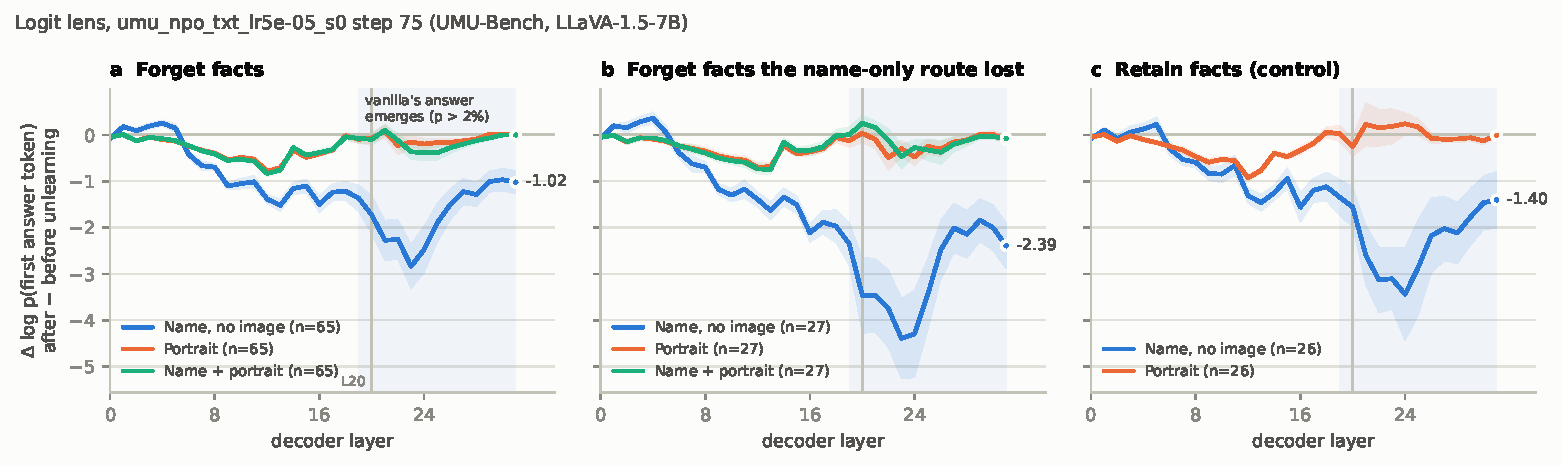
\includegraphics[width=\linewidth]{figures/lens_step75.pdf}
\caption{Logit lens of the unlearned model minus the vanilla, by decoder layer, for the first token of the
correct answer (mean $\pm$1 SEM over doubly-correct facts). (a) all forget facts; (b) the forget facts the
name-only route answered wrongly at this step; (c) retain facts. Shaded: layers where the vanilla starts to
assign the answer more than 2\% (from layer 19). Vertical line: layer 20, where image identity is resolved in
LLaVA-1.5-7B~\cite{cohen2024}. Run with forget-only NPO, lr $5\times10^{-5}$, step 75 of 300.}
\label{fig:lens}
\end{figure}

\paragraph{What the lens shows (Fig.~\ref{fig:lens}).}
\begin{enumerate}
\item \textbf{The text route is suppressed where the answer forms.} The name-only route reaches its lowest
  point at layer 23 ($\Delta\log p = -2.84$; $-4.40$ on the 27 facts it got wrong behaviourally), inside the
  layers where the vanilla starts to produce the answer.
\item \textbf{The image route is barely touched in those layers} ($-0.19$ averaged over layers 22--24) and ends
  at $-0.02$. This argues against the strong form of \Htwo: there is no comparable suppression for later
  layers to compensate.
\item \textbf{Adding the portrait to the name-based question removes the suppression.} The name + portrait
  curve follows the portrait curve, not the name curve (final layer $0.00$ vs.\ $-1.02$). In this checkpoint
  the gate is not the name. Either the absence of an image is the trigger, or, with an image present, the
  model identifies the person from the image and ignores the name.
\end{enumerate}

\paragraph{What the lens does not show.}
\begin{itemize}
\item \Hone{} versus \Honep: the lens shows where an effect becomes visible in the output basis, not where the
  LoRA acts. An early edit would also first appear in these layers.
\item A fact-specific mechanism: the retain text route is suppressed with the same profile
  (layer 23: $-3.10$). Much of the curve may describe ``text-only input is suppressed'' rather than ``these
  facts are forgotten''.
\item The small early dip of both image routes around layer 12 ($\approx -0.8$): the vanilla gives the answer
  about $e^{-7}$ there, the logit lens is unreliable at that depth, and the retain image route shows the same dip.
  Weak compensation is neither supported nor excluded.
\item Generality: one seed, one checkpoint five steps before collapse, bf16, and a vanilla that never saw an
  input without an image. That last point makes ``no image'' an easy feature for NPO to latch onto and may
  not hold for a model trained on both forms.
\end{itemize}

\paragraph{Status of the hypotheses.}
Strong \Htwo: disfavoured. \Hone: the input-form gating part fits, but the form feature is the absence of the
image rather than the name, and the late-layer part is untested. \Honep: untested; if its core is an edited
early name pathway, the unaffected name + portrait route is evidence against it, not yet decisive.

%===========================================================================================================
\section{Plan}
\label{sec:plan}

Each step has a decision attached; the order puts the cheapest decisive test first.

\begin{enumerate}
\item \textbf{Specific unlearning (run 2, ready).} NPO plus a retain NLL term on text-only questions of 50 other
  people (disjoint from the retain readout), lr $2\times10^{-5}$, two epochs, evaluated every half epoch with the
  name + portrait form and a degeneracy check. \emph{Decision:} if name + portrait is now suppressed, the gate has
  moved to the name; if not, ``an image present bypasses the forgetting'' is robust to specificity.
\item \textbf{Image-swap test.} Name-based question with another person's portrait, and with a blank image.
  \emph{Decision:} suppression gone for both $\Rightarrow$ the gate is image presence; present with another
  person's portrait $\Rightarrow$ identity from the image overrides the name.
\item \textbf{LoRA layer masking.} Keep the unlearning LoRA on early or late layers only.
  \emph{Decision:} removing late layers restores text answers $\Rightarrow$ \Hone; only removing early layers
  does $\Rightarrow$ \Honep.
\item \textbf{$\lVert\Delta W x\rVert$ by token group} (name / image / template / last) for name-only versus
  name + portrait inputs. \emph{Decision:} similar on name tokens in both inputs but only one suppressed
  $\Rightarrow$ name tokens are not the trigger.
\item \textbf{Cross-route patching} of late text-route states into the image run (after the fp32 tool checks).
\item \textbf{Asymmetry.} The reverse condition (portrait-based unlearning) and the same tools; compare where the
  two gates sit.
\item \textbf{Robustness and confound.} A second seed and learning rate; a larger retain readout (100 people)
  and the real-person set at the selected checkpoint; re-score the archived Qwen2-VL vanilla with the generation
  readout; if the ``no image'' confound persists, fine-tune a vanilla with genuine text-only questions using
  UMU-Bench's recipe.
\end{enumerate}

\paragraph{Timeline} (target: ARR January 2027 cycle; dates to confirm).
\begin{center}
\small
\begin{tabular}{@{}ll@{}}
\toprule
Weeks & Work \\
\midrule
Nov 5--11 & Run 2; image-swap test; fp32 tool checks \\
Nov 12--25 & LoRA masking, $\lVert\Delta Wx\rVert$; decide \Hone{} vs.\ \Honep \\
Nov 26--Dec 9 & Cross-route patching; reverse (image) unlearning; asymmetry analysis \\
Dec 10--23 & Seeds, learning rates, larger retain and real-person evaluation; vanilla confound check \\
Dec 24--Jan & Writing; figures; buffer \\
\bottomrule
\end{tabular}
\end{center}

\section{Risks}
\begin{itemize}
\item \textbf{Fine-tuned fictitious knowledge.} Knowledge injected by fine-tuning is removed more easily than
  pre-trained knowledge~\cite{deeb2024}; conclusions may not transfer to real entities. Mitigation: a real-entity
  check on UNLINK-VL~\cite{unlinkvl} if time allows.
\item \textbf{The vanilla never saw text-only inputs.} The leak may partly be a format effect specific to this
  checkpoint. Mitigation: plan steps 1, 2 and 7.
\item \textbf{Unlearning instability.} Forget-only NPO collapsed within two epochs. Mitigation: retain term,
  lower learning rate, half-epoch checkpoints, degeneracy monitoring.
\item \textbf{Small samples.} 65 forget and 26 retain doubly-correct facts. Mitigation: larger retain readout at
  the selected checkpoint; \texttt{forget\_15} if more forget facts are needed.
\end{itemize}

%===========================================================================================================
\begin{thebibliography}{99}\small
\bibitem{umubench} C.~Wang, Y.~Li, X.~Feng, C.~Chen, X.~Zheng, J.~Yin.
  UMU-Bench: Closing the Modality Gap in Multimodal Unlearning Evaluation. NeurIPS 2025 Datasets and Benchmarks Track.
\bibitem{mllmu} Z.~Liu et al. Protecting Privacy in Multimodal Large Language Models with MLLMU-Bench.
  arXiv:2410.22108. % VERIFY author list and venue
\bibitem{llava15} H.~Liu, C.~Li, Y.~Li, Y.~J.~Lee. Improved Baselines with Visual Instruction Tuning. arXiv:2310.03744.
\bibitem{npo} R.~Zhang, L.~Lin, Y.~Bai, S.~Mei. Negative Preference Optimization: From Catastrophic Collapse to
  Effective Unlearning. arXiv:2404.05868.
\bibitem{unlinkvl} UNLINK-VL. arXiv:2608.03791. % VERIFY: full title and authors (research.md notes inconsistent author lists)
\bibitem{smu} SMU. arXiv:2607.18615. % VERIFY full reference
\bibitem{idunlearn} IDUnlearn-Bench. arXiv:2609.33481. % VERIFY full reference
\bibitem{crossinf} CrossInf. arXiv:2607.16442. % VERIFY full reference
\bibitem{pava} PAVA. arXiv:2608.30649. % VERIFY full reference
\bibitem{uds} UDS. arXiv:2605.24614. % VERIFY full reference
\bibitem{hong2024} Y.~Hong et al. Intrinsic evaluation of unlearning using parametric knowledge traces.
  arXiv:2406.11614. % VERIFY: research.md cites 2410.06606 (MLP coefficients) and 2406.11614 (ConceptVectors)
\bibitem{guo2024} P.~Guo et al. Mechanistic unlearning: robust knowledge unlearning and editing via mechanistic
  localization. arXiv:2410.12949. % VERIFY
\bibitem{cohen2024} I.~Cohen et al. Performance gap in entity knowledge extraction across modalities in vision
  language models. arXiv:2412.14133. % VERIFY
\bibitem{nikankin2025} Y.~Nikankin et al. arXiv:2506.09047. % VERIFY full reference
\bibitem{deeb2024} A.~Deeb, F.~Roger. Do unlearning methods remove information from language model weights?
  arXiv:2410.08827. % VERIFY
\end{thebibliography}

\end{document}
